\chapter{Methodology}
\section{Project Scope \& Goal}
The project scope had to have a system with several functioning parts that worked with as many modern technologies as possible. Original ideas for this project paralleled the ideas of Desktop Application Development and Game Development. These possible routes for the project were researched with the focus on UI (User Interface) and experience. One of these ideas was a desktop application for people to send Curriculum Vitaes (CV) to relatable companies. On this suggested app, the user would upload their CV. That CV would be sent through an A.I. (Artificial Intelligence) system that would read it, pick out the keywords and send it to companies looking for future employees in that field. At first, this was a great concept but constructing an app for this service was an extensive scope as it would have to either have a vast database or a third party API to correlate all the companies from different sources.
\\\\ Another initial idea was to develop a fully-fledged open-world Game in the Unreal Engine with C++. This idea was drastically different from the others due to it originating from a creative perspective and personal interest. Old noir films and parallel universes inspired the game. Making a mix of these two genres would be quite exciting and would mean that this open-world would have to be huge. This idea was a favourite and unfortunately had to be forfeited as it was overly ambitious. Perhaps, this project will be pursued in the future with a time allocation to permit it. 
\\\\ In the end, it was decided to develop a service report application for automobile technicians. This would include an app that allowed service reports to be completed for auto dealerships and rental companies. This idea was considered through observations of my brother's line of work which specializes in the supply and service of new and used Mobile Plant and Equipment. The company found challenges when documenting service reports on paper and Microsoft Excel. Initially, the app was to be a desktop app but after consideration, it transpired that it would would be most suitable to work on a tablet or a mobile phone. With this, the Angular and Ionic framework was chosen for the front-end to build it into a website app. The app needed to ensure confidentially and security as it would include sensitive, work-related data. Therefore, the desktop app focus was not ideal as some app's data may need to be temporarily held on the computer running it. This would make the data less secure than if it were on a back-end database server. \cite{ref1}
\\\\ This app would need a quick and robust back-end to provide the front-end's users with time efficient and immediate connection to the database. Google's relatively new language Golang (Go) to implemented the functionality of it and OpenAPI to design the API environment to connect the the back to the front-end were chosen. Go is based off the C programming language and is proven to be as prompt as other languages such as Java and C++. There are several web frameworks for Go available, such as Gorilla Mux, Martini and Gin Gonic. After researching and testing, Gin proved to be the best web framework to use as it consists of the necessary requirements for CORS (Cross-Origin Resource Sharing) requirements. In conclusion, Go with Gin was the most suitable choice for the back-end component of the application.
\\\\ A reliable and strong database was essential as this project's focus was for the application to have the ability to be used in a working environment; it would have to store a large quantity of data that needed to be accessed quickly and be able to add and update the data freely from the front-end through the connection of the back-end. MySQL was chosen for the database as it is proven to have these mentioned qualities with its use of schemas and InnoDB transactions. 
\\\\ The entire application would need to be hosted through a cloud platform to achieve the SaaS requirements. AWS (Amazon Web Services) provides a first year free tier. AWS would be an adequate platform for hosting the application as it has a wide range of services. The ideal setup for the hosting would be S3 Bucket for the front-end, Elastic Beanstalk for the back-end and an EC2 Ubuntu Virtual Machine for the database.

\section{Development Methodology}
The planned approach for the development method was the Agile methodology, Personal Scrum, which consisted of plans and implementations that allowed for flexibility and adaption. Waterfall was considered as it would be ideal to have everything planned and documented before implementation. However, with new frameworks and technologies, Waterfall was not suitable as some problems could arise with these unfamiliar frameworks and technologies. With the use of Personal Scrum, the project was separated into sprints to focus on robustness more than anything else. This section's remainder discusses why and how this approach benefited the development and shows how a Waterfall approach was not suitable. Also, Figure 2.1 shows how Waterfall and Agile structure projects.

\subsection{Waterfall}
Waterfall is based on Civil Engineering and how software packages for spacecraft mission planning, commanding, and post-flight analysis were developed. \cite{ref2} It requires almost a complete prediction of the project with a "Big Design Up Front" from planning and documenting the development process. Before coding, the project manager makes a plan and then writes detailed documentation of all plan phases. These phases happen in a strict order. \cite{ref3}
\\\\ \textbf{The Five Phases of Waterfall Life-cycle}
\begin{itemize}
    \item Requirements Analysis and Specification
    \item Architectural Design
    \item Implementation and Integration
    \item Verification/Testing
    \item Operation and Maintenance
\end{itemize}

With Waterfall, each stage is required to be fully completed before the next one is attended. This project has a setup of a Front-end and Back-end, meaning if Waterfall were used, it would have most likely required the back-end to be completely built before the front-end was ever touched. This process is not ideal as some cross-origin issues (CORS) can happen between both ends and result in refactoring the back-end in order for it to be able to connect to the front.

\subsection{Agile}
Agile project management and software development is an iterative approach that enables teams to be flexible and adaptable. This method allows for versatility and, depending on the project, allows for delivering a valuable product to consumers faster and without the upfront requirements with Waterfall. Agile employs the Scrum framework, which involves sprints that are fixed-length work iterations. Each sprint has four ceremonies that provide structure. \cite{ref4}
\\\\ \textbf{The Four Ceremonies of Scrum}
\begin{itemize}
    \item Sprint Planning
    \item Sprint Review
    \item Sprint Retrospective
    \item Daily Scrum
\end{itemize}

\subsection{Personal Scrum}
Personal Scrum is an Agile methodology that employs scrum practices for one-person projects; through observation of what work has been fulfilled, adaptation of work that requires refactoring, incremental elaboration for planning, prioritizing and sizing of the essential work with the use of allocated time-frames to improve personal productivity. \cite{ref5}
Dustin Wax, executive director at Burlesque Hall of Fame, states that scrum is intended for "big, collaborative projects" yet it can be applied to "individual productivity" just as well. \cite{ref5}
 
Having this approach allowed to have 1-2 days a week to block out other college work and have them dedicated to the project. These days were usually allocated to the end of the week and during college time off, more days were designated to increase productivity time. The first day mainly consisted of a review the week previous' work, plans and setups for implementations to be done the next day. On the second, if the implementations were either finished or in part, the project's supervisor was informed of the progress, any problems that occurred, and what was next to be done.

\begin{figure}[H]
    \caption{Agile VS Waterfall}
    \label{image:agileVSwaterfall}
    \centering
    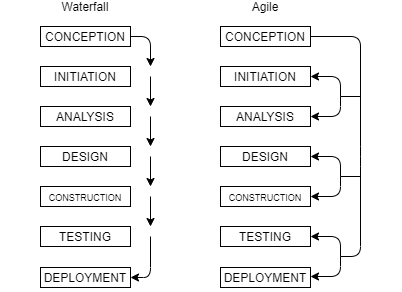
\includegraphics[width=0.72\textwidth]{images/misc/agile-vs-waterfall.png}
\end{figure}

\subsection{Project \& Time Management}
In order to have a structured schedule for the project, this required a tracking software with a scrum board. Softwares such as Jira and YouTrack were considered, which seemed a bit over the top for a one-person project. GitHub's repositories have a section titled 'Projects' (Figure 2.2). Here a work board for the repository can be created to organize the work into cards. GitHub issues can be referenced to allow a card to keep track of a particular issue. GitHub's Projects was very convenient, especially with it being in the project's repository. GitHub Issues (Figure 2.3) are a way of tracking enhancements and any problems encountered for projects and are also located in the project's repository.

\begin{figure}[!ht]
    \caption{GitHub Projects}
    \label{image:gitProjects}
    \centering
    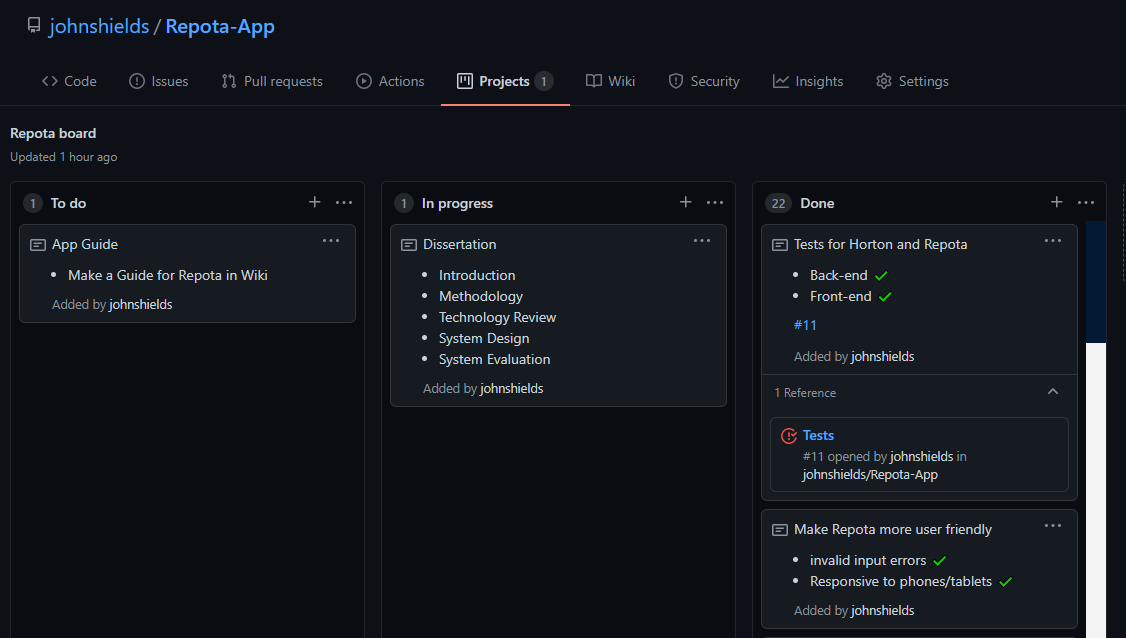
\includegraphics[width=0.8\textwidth]{images/misc/git-projects.png}
\end{figure}

\begin{figure}[!ht]
    \caption{GitHub Issues}
    \label{image:gitIssues}
    \centering
    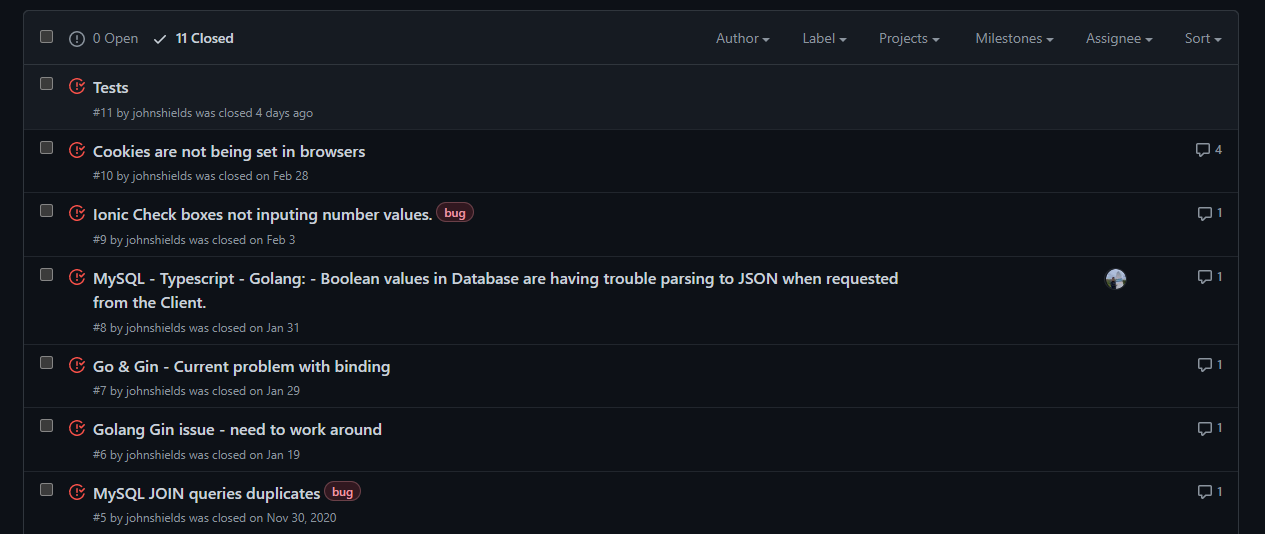
\includegraphics[width=0.8
    \textwidth]{images/misc/git-issues.png}
\end{figure}

\subsection{Verification \& Testing}
In order to get the project set up, a prototype MySQL database was structured with just an automobiles table. Then a basic Go back-end with the web framework Gorilla Mux was set up to have access to that database. Next was a simple Angular and Ionic front-end that connected to the back-end to present that table on a history page of reports. The first issue was that data from the back-end was unable to cross over to the front-end due to CORS. In order to resolved this issue the web framework was changed to Gin Gonic to allow a CORS function to be implemented into the back-end to resolve this issue. Once that was all implemented, an AWS E2C Ubuntu Virtual Machine (VM) was initiated to host the database and the back-end. With the server now in the project, the front-end was altered to connect to the back-end running on the VM. This initial setup fined tuned the environment which, allowed the real development to begin. 

\subsubsection{Integration and High-level Behavior Tests}
To make sure the back-end and front-end were robust, tests were written. Go's standard package for testing was used to perform integration tests for tests on multiple operations of the back-end at the same time. While CucumberJS was chosen to test the high-level behavior of the front-end which, tests it from a user's perspective. These tests are explained further in the System Evaluation chapter.

